\documentclass{article}
\usepackage[utf8]{inputenc}
\usepackage{fullpage}
\usepackage{float}
\usepackage{graphicx}
\usepackage{gensymb}
\usepackage{amsmath}
\usepackage{amssymb}

\title{Chapter 8: Image Theory Application}
\author{Rohit Singh}
\date{June 2022}

\begin{document}

\maketitle

\section{Course Notes}

\subsection{Image Theory}

\textbf{Definition} Image theory says that a charge (point or distributed) lying above a perfectly conducting surface gives the same field as in the case where the surface is removed and an image charge (equal magnitude, opposite sign) is positioned symmetrically with respect to the surface.

\begin{figure}[H]
  \centering
     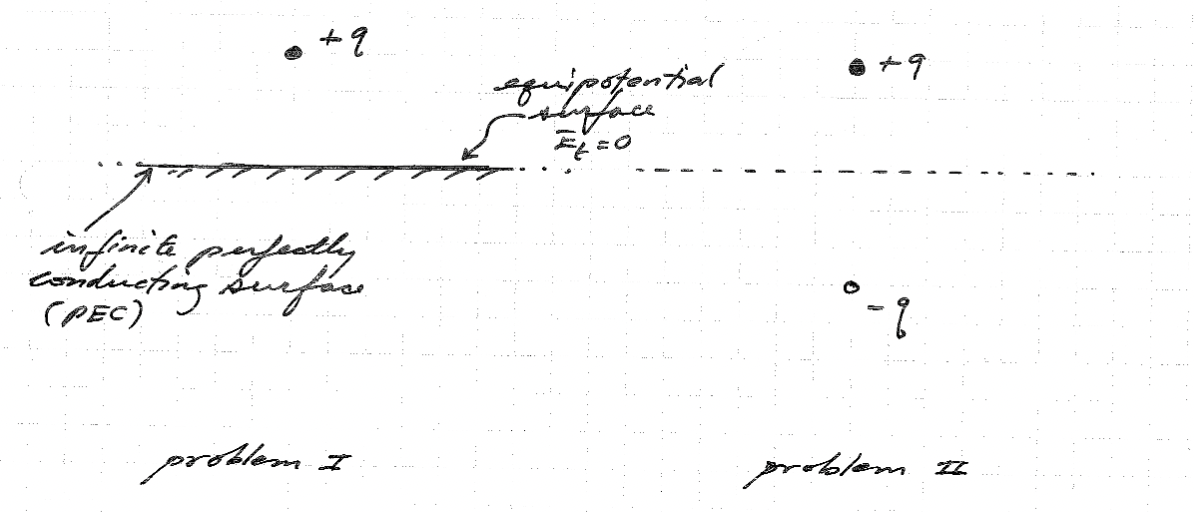
\includegraphics[scale=0.8]{Course Notes/images/8.1.png}
  \caption{A charge over a PEC (problem 1) and it's image theory equivalent (problem 2)}
\end{figure}

We can replace the static charges with dynamic charges such as current and can use the graphical method to deduce current images.

With the graphical method, we consider the vector of the dynamic charge, and when we image the current, the horizontal component is equal in magnitude \textbf{but opposite in sign}, and the vertical component is equal in magnitude \textbf{and equal in sign}

\begin{figure}[H]
  \centering
     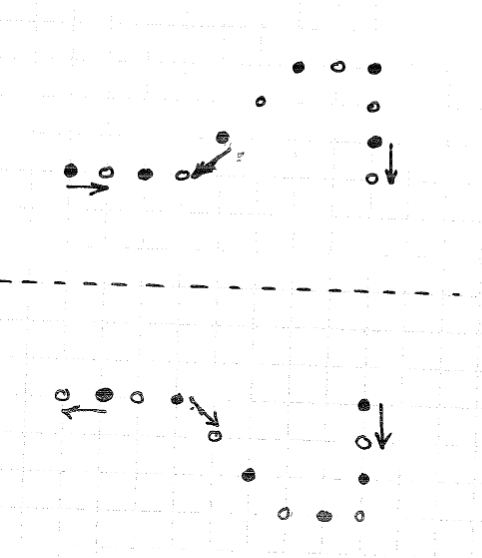
\includegraphics[scale=0.8]{Course Notes/images/8.2.png}
  \caption{A current and it's imaged counterpart, with vectors showing movement}
\end{figure}

Remember that the assumption for the image theory to hold is that the conducting place must be \textbf{infinity} and \textbf{perfectly conducting}

By looking at figure 2, we see something interesting happens in the horizontal component that is similar to the current distribution in a dipole antenna, that is, current flowing along the entire vertical length in the same direction. This allows us to define a monopole antenna in reference to a dipole antenna.

\subsection{Monopole Antenna}


\begin{figure}[H]
  \centering
     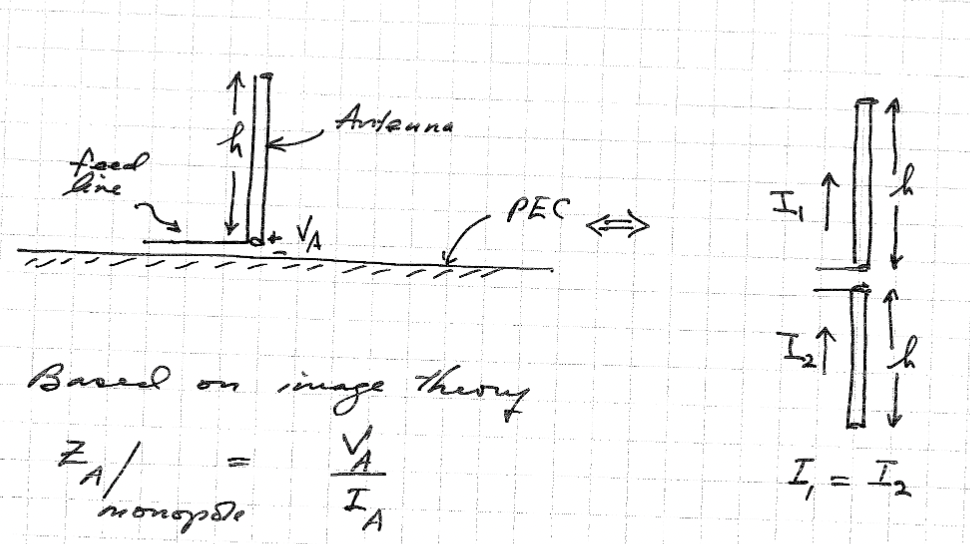
\includegraphics[scale=0.8]{Course Notes/images/8.3.png}
  \caption{A monopole antenna and its dipole antenna imaged equivalent}
\end{figure}

From figure 3, we see that a monopole antenna radiating over a ground plane is equivalent to a dipole antenna radiating in free space!

The charge distribution on the monompole is equivalent in both cases, from which we can see that the current into the monopole is the same as the current flowing in the entire dipole.

The voltage however, is not that same, due to the difference in the voltage gap feed, giving us:

\begin{center}
    $V_A = \frac{1}{2}V_D \implies Z_{A, mono} = \frac{1}{2} Z_{A, dipole}$
\end{center}

From this, we can see that the power of the monopole is half the power in the dipole, which makes sense since the power is radiated in one hemisphere instead of two.

\subsection{Duality}

Let us define system 1 such that:

\begin{center}
    $\triangledown \times \Vec{E}_1 = -j \omega \mu_1 \Vec{H}_1$ \\ 
    \hspace{0.1} \\
    $\triangledown \times \Vec{H}_1 = j \omega \epsilon_1 \Vec{E}_1 + \Vec{J}_1$ \\ 
    
\end{center}

To determine the \textbf{duality} between two systems, we consider system 1 which consists of an electric current source $\Vec{J}_1 \ne 0$ (can be an infinitesimal source or a distribution over some finite support), and no magnetic current source, ($\Vec{M}_1 = 0$)

Now, consider a new system, system 2, such that:

\begin{center}
    $\triangledown \times \Vec{E}_2 = -j \omega \mu_2 \Vec{H}_2 - \Vec{M}_2$ \\ 
    \hspace{0.1} \\
    $\triangledown \times \Vec{H}_2 = j \omega \epsilon_2 \Vec{E}_2$ \\ 
\end{center}

Unlike system 1, system 2 has a magnetic current source, $\Vec{M}_2 \ne 0$, and no electric current source $\Vec{J}_2 = 0$

Now, to consider the duality of the two systems, we must do the following:

\begin{enumerate}
    \item Observe the similarity between the two systems
    \item Replace $(\mu_2, \epsilon_2)$ in system 2 with $(\epsilon_1, \mu_1)$ 
    \begin{center}
    $\triangledown \times \Vec{E}_2 = -j \omega \epsilon_1 \Vec{H}_2 - \Vec{M}_2$ \\ 
    \hspace{0.1} \\
    $\triangledown \times \Vec{H}_2 = j \omega \mu_1 \Vec{E}_2$\\ 
\end{center}
    \item Let $\Vec{M}_2 = \Vec{J}_1$ in magnitude, orientation and distribution
    \begin{center}
    $\triangledown \times \Vec{E}_2 = -j \omega \mu_2 \Vec{H}_2 - \Vec{J}_1$ \\ 
    \hspace{0.1} \\
    $\triangledown \times \Vec{H}_2 = j \omega \epsilon_2 \Vec{E}_2$ \\ 
\end{center}
\end{enumerate}

If we compare system 2 with system 1, we see that they are completely identical \textbf{if and only if}:

\begin{center}
    $\Vec{E}_2 = -\Vec{H}_1$ and $
    \Vec{H}_2 = \Vec{E}_1$
\end{center}

From this, we can conclude that system 2 can be obtained from system 1 if the following substitutions are made:

\begin{center}
    $\Vec{J}_1 \to \Vec{M}_2$ \\
    $\Vec{H}_1 \to -\Vec{E}_2$ \\
    $\Vec{E}_1 \to \Vec{H_2}$ \\
    $\mu_1 \to \epsilon_2$ \\
    $\epsilon_1 \to \mu_2$
\end{center}

Using the same logic, we can construct a magnetic line current by staggering many loops in succession.

Through some logic, we can see that the solution for a small loop \textbf{in free space} follows from the solution of the infinitesimal Herzian current \textbf{in free space}

\subsubsection{Use of Duality}

Magnetic current does not exist in nature since a magnetic charge is not possible. However, let us assume there is such a thing as a \textbf{magnetic dipole} with a field distribution analogous to that of the electrical dipole. This would result in a magnetic force/field distribution looking like:

\begin{figure}[H]
  \centering
     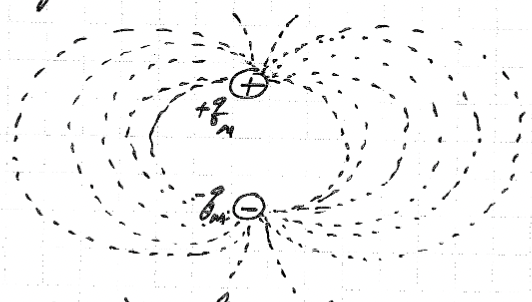
\includegraphics[scale=0.8]{Course Notes/images/8.4.png}
  \caption{Magnetic field lines of a magnetic dipole}
\end{figure}

A physical situation that closely emulates this behavior is a system with a small loop carrying a constant current $I$

\begin{figure}[H]
  \centering
     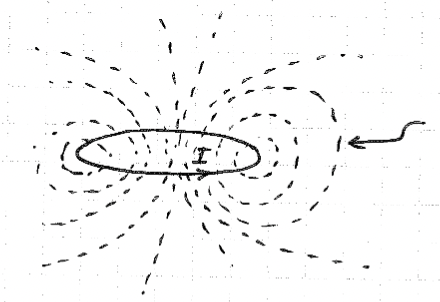
\includegraphics[scale=0.8]{Course Notes/images/8.5.png}
  \caption{Magnetic field lines of a small loop with current $I$}
\end{figure}

Notice the similarities between the two systems, from which we conclude that the small loop is an equivalent system to the magnetic dipole.

\subsection{Small loop Antenna}

The qualtitative radiation characteristics of a small loop were derived using duality. Another approximation that allows us to derivce important quantitiative characteristics such as input impedance is the square loop approximation. Using this model, we can use the vector potential method to obtain a square loop antenna from the ideal circle loop antenna. The math is left in the lecture notes rather than being re-written here.

\section{In Lecture Notes}

We are motivated in the study of image theory for a few reasons:

\begin{itemize}
    \item Consider point-to-point communication between two transmitters a far distance away.
    \begin{itemize}
        \item Although we expect the signal to be transmitted from one dish straight to another, we actually have rays coming from many directions, such as onces bouncing off the ground, planes, etc.
        \item The rays bouncing of the ground can be strongly affected by the material that is on the ground, such as sand, wet sand, etc.
        \item So far, we do not know how to solve an antenna over a ground plane like in this situation, so what do we do?
    \end{itemize}
\end{itemize}

If we have a charge on top of an \textbf{infinite perfectly conducting surface} (PEC), this is equivalent to having a charge on top of the surface with an equal and opposite charge the same distance below the surface, with no PEC. This allows us to solve problems with an antenna over a ground plane by simply throwing away the PEC and treating the problem as if it is radiating in free space!

We can leverage superposition to extend this scenario to more complex ones, in which there are multiple charges distributed over a PEC. 

We can further leverage this in the case of a horizontal current flowing between points $A \to B$ above the PEC, which would be \textit{imaged} below the surface as an equal current flowing between points $B \to A$, which is unintuitive but makes sense when we consider that it is \textit{equal and opposite}.

However, this is not the case if the current is going vertically, in which case the imaged current is equal and travelling in the same direction as the original current. For the neither horizontal or vertical case, the x (horizontal) component is flipped but the y (vertical) component is not.

We leverage this vertical component to design \textbf{monopole antennas}, which can be seen as a dipole antenna reverse-imaged (cut in half) and put over a PEC.

\end{document}